%%
%% Template chap1.tex
%%

\chapter{Background}
\label{cha:background}

\section{First Order Logic Terms and Notation}
\label{sec:terminology}

This thesis focuses around the extension of \beagle, a \emph{first order logic} (FOL) theorem prover.
Specifically \beagle\ operates on first order logic \emph{with equality}, where the only
true \emph{predicates} (boolean functions) are $=$ (the equality operator), $\lor$ (logical OR),  and
$\lnot$ (negation). Other predicates (including $\land$, the logical AND operator) can be defined
in terms of these three operations.
In order to understand beagle's purpose and functions a basic understanding of first order logic
with equality is required; but for reference a brief glossary of important terminology used throughout the paper
is provided here.

\subsubsection{Logic Expressions}

\begin{itemize}
\item \textbf{Variable:} A general symbol which may be replaced by another term.
\item \textbf{Function Symbol:} Functions with an \emph{arity} describing how many
arguments they take. Arity 0 functions are referred to as \emph{constants}.
\item \textbf{Term:} An expression made up entirely of function applications and variables.
\item \textbf{Subterm:} A term contained within another term.
\item \textbf{Equation:} an \emph{equality} statement, such as $s = t$ where $s$
and $t$ are terms. Equations can be used to \emph{emulate} other predicates
by adding reserved constants for \emph{true} and \emph{false}. For example $isEmpty(s) = true$.
\item \textbf{Literal:} An equation or a \emph{negated} equation. For example $\lnot (s = t)$,
written $s \neq t$.
\item \textbf{Clause:} Throughout this paper we use clause to refer specifically to a \emph{conjunctive normal form} clause,
which is a collection of literals joined with $\lor$.
\end{itemize}

\subsubsection{Logic Calculus}

A \emph{calculus} refers to a set of rules which can be used to infer new information
from a knowledge base; usually by combining two or more clauses.

\subsubsection{Soundness and Completeness}

A logical calculus may be \emph{sound} and/or \emph{complete}. A calculus
is sound if it cannot be used to derive an expression which is not truly a theorem.
A calculus is complete if it can be used to derive all true theorems in any logical
system. Incomplete calculi can occasionally be useful in special cases; but unsound
calculi are generally useless.

\subsubsection{Positions}
Many concepts in this paper require the ability to precisely point out a specific
subterm/symbol within a term. Thus we introduce a syntax for term \emph{positions}.
This sort of syntax is a standard concept in the field of logic; but here we
will be using a slightly extended syntax as we will have need to reference
positions which do not exist \cite{shulz12}.

A \emph{position} is given as a (possibly empty) list of natural numbers.
$t|_p$ refers to the subterm of $t$ at position $p$.
The empty position, $t|_\epsilon$, refers to the outermost function or variable
of a term. A position $t|_n$ refers to the $n^{th}$ argument of the outermost function,
$t|_{n.m}$ to the $m^{th}$ argument of that $n^{th}$ argument; and so on. If the position
does not exist in the term we return Nil. Consider the following example:
\[t = f(a, g(a, x, y), b)\]
\[t|_{\epsilon} = f \quad\quad t|_{1} = a \quad\quad  t|_{2.2} = x \quad\quad  t|_{2.3.3} = \text{Nil} \quad\quad  t|_{3.2} = \text{Nil}\]

\subsubsection{Substitutions}

A \emph{substitution} is a function which replaces one or more variables in an expression
with another term. Substitutions are required to define two important relations between
expressions:

\begin{itemize}
\item \textbf{Unification:} expressions $s$ and $t$ are \emph{unifiable} if there exists a substitution
$\sigma$ such that $s\sigma = t\sigma$. Unifiable terms will have a unique \emph{most general unifier} (mgu).
\item \textbf{Subsumption:} an expression $s$ \emph{subsumes} $t$ if there exists a substitution
$\sigma$ such that $s\sigma = t$. This can also be stated as $t$ is an \emph{instance} of $s$.
\end{itemize}

%\subsection{Popular Problems in First Order Logic}

\subsection{The Superposition Calculus}
\label{sec:supcalc}

\cite{supcalc} \cite{smartmatch}

\begin{align*}
\textbf{Positive Superposition} &&& \frac{l \approx r \lor C\quad \quad s[u] \approx t \lor D}{(s[r] \approx t \lor C \lor D)\sigma}
\intertext{\tcent{Where $\sigma = $ mgu $(l,u)$ and $u$ is not a variable}}
\textbf{Negative Superposition} &&& \frac{l \approx r \lor C\quad \quad s[u] \not\approx t \lor D}{(s[r] \not\approx t \lor C \lor D)\sigma}
\intertext{\tcent{Where $\sigma = $ mgu $(l,u)$ and $u$ is not a variable}}
\textbf{Equality Resolution}    &&& \frac{s \not\approx t \lor C}{C\sigma}
\intertext{\tcent{Where $\sigma = $ mgu $(s,t)$}}
\textbf{Equality Factoring}     &&& \frac{l \approx r \lor s \approx t \lor C}{(l \approx t \lor r \not \approx t \lor C)\sigma}
\intertext{\tcent{Where $\sigma = $ mgu $(s,l)$}}
\end{align*}


\section{Automated Reasoning and Theorem Proving}
\label{sec:proving}

Automated Reasoning is a rapidly growing field of research where computer programs
are used to solve formal logic problems; typically stated in first order logic.
The most common variety are \emph{resolution} provers. These take as input a knowledge
base of theorems and a \emph{query} logic statement. The query can be proven a theorem
by adding its \emph{negation} to the knowledge base and repeatedly attempting inference rules
until arriving at a contradiction.

Some existing resolution theorem provers include:

\begin{itemize}
\item \textbf{SPASS}
\cite{spass}
\item \textbf{Vampire}
\cite{vampire}
\item \textbf{E}
\cite{eprover}

\end{itemize}

\section{Term Indexing}
\label{sec:indexing}

Term indexing is a technique used to better locate clauses and terms for which inference rules
in a calculus will apply. In particular, these indices are used to find all terms which
will or are likely to \emph{unify} with, \emph{subsume} or be subsumed by a query term. These relations are typical conditions
of first order logic inference rules, for example all rules for the superposition calculus
in Section \ref{sec:supcalc} require some unifier $\sigma$.
The process of implementing Term Indexing forms the core of this paper. Our goal
is to implement a recent technique known as Fingerprint Indexing (see Section \ref{sec:fingerprint});
but for examples and comparison we present here some other techniques.
Refer to \cite{indexing} for more detailed specifications of these techniques along
with some results comparing them.

\subsubsection{Top Symbol Hashing}
Top symbol hashing simply compares the outermost symbol of any two terms and checks
that they are compatible. For example, for the term $f(a,x)$ it would simply look
at the symbol $f$ and present any other term with the top symbol $f$ (or a variable) as compatible.
All terms compatible in this manner could be retrieved instantly with a standard
single layer hash map.

Top symbol hashing is provided as a simple example; it is very rudimentary and
is certainly not in active use by any popular theorem provers.

\subsubsection{Discrimination Trees}

Discrimination Trees work by storing terms in a tree at a position determined by the structure
of each term. Each branch in the tree has a label which is either a function symbol
(e.g. $f$, $g$) or *, which may represent any variable. To place a term in the tree
we traverse the term from left to right and follow or create branches according to
which symbol we observe. This process is simple. but retrieving from the index is a
complex process requiring a backtracking algorithm.

This technique can be extended by keeping track of variable names; as opposed to
replacing them all with a *. This extension makes Discrimination Trees a \emph{perfect} indexing technique in that anything
returned by the indexer is guaranteed to be unifiable\cite{mccune}. While this extension sounds
ideal, in practice it can result in a large index which takes
a considerable amount of time to retrieve terms. This performance
loss is often enough to offset any gain from implementing perfect indexing.

Discrimination Trees have another distinct disadvantage in that their tree data
structure can grow arbitrarily large depending on the size and variety of observed terms.

\subsubsection{Path Indexing}

Path Indexing is currently in active use in the Vampire theorem prover \cite{vampire}.
It behaves similarly to Discrimination Trees but rather than mapping out entire terms
it only maps a selection of \emph{paths}. A path in a term is a lists of function symbols
ending in a variable or constant, generated by following an argument of each function application.
For example there are two paths in $f(g(h(a), x))$, $[f, g, h, a]$ and $[f,g,x]$.

Terms are stored in a tree structure according to which paths they possess; and retrieval
is performed by finding terms in the tree which have compatible paths. This process
is not straightforward and requires a backtracking algorithm with repeated use of
the costly set intersection operation.

\section{Fingerprint Indexing}
\label{sec:fingerprint}

\emph{Fingerprint Indexing} is a recent technique developed by \citeN{shulz12}, the creator
of the E prover. It works by computing a \emph{fingerprint} for each logic term;
which can then be compared for unification or match compatibility. 
Like most of the example techniques above,
Fingerprint Indexing is \emph{non-perfect} in that compatible fingerprints will not
always imply that the associated terms successfully unify/match. The technique
makes up for this by being adjustable to arbitrary levels of precision; ranging between
what essentially amounts to Top-Symbol Hashing (See section \ref{sec:indexing})
to comprehensive, but slow to compute, term comparisons.

\subsection{Term Fingerprints}
\label{sec:fingerprints}

A term's \emph{fingerprint} is a list of \emph{fingerprint features} which
indicate what the term looks like at a given position. The 4 possible
fingerprint features are:
\begin{itemize}
\item $f$ (any function or constant in the current system): The term has an application of $f$ at the given position.
\item \textbf{A}: The term has a variable at the position.
\item \textbf{B}: The position does not exist in the term, but can be created
by expanding a variable via substitution.
\item \textbf{N}: The position does not exist and cannot be created.
\end{itemize}
Term fingerprints are computed with respect to a list of positions; by
computing which feature exists at each position. We will now revisit the example from
the explanation of term positions (in Section \label{sec:terminology}) to show
the computation of a fingerprint. In the example $\{f,g\}$ are functions, $\{a,b\}$ are
constants and $\{x,y\}$ are variables.
\[t = f(a, g(a, x, y), b)\]
\[\text{positions} = [\epsilon, 1, 2.2, 2.3.3, 3.2] \]
\[t|_{\epsilon} = f \quad\quad t|_{1} = a \quad\quad  t|_{2.2} = x \quad\quad  t|_{2.3.3} = \text{Nil} \quad\quad  t|_{3.2} = \text{Nil}\]
\[\fp(t, \text{positions}) = [f, a, \textbf{A}, \textbf{B}, \textbf{N}] \]

\subsection{The Fingerprint Index}
\label{sec:fpindex}

Once a term's fingerprint has been generated we use it to store the term in a tree-like
data structure known as the \emph{Fingerprint Index}. 
This data structure is very reminiscent of a Discrimination Tree (See section \ref{sec:indexing})
and works similarly. To add a term to the index we (starting from the root node) follow/create
branches labelled with the fingerprint features of the term's fingerprint. Once the fingerprint has run
out we store the term in a leaf set. Figure \ref{fig:fpindex} presents an example Fingerprint
Index; built by sampling positions $\epsilon$, 1 and 2 for a variety of terms.

\begin{figure}[H]
  \centering
  \includegraphics[page=7,width=0.9\textwidth,trim=5cm 14.3cm 4.8cm 4.5cm,clip]{resources/schulz}
  \caption
   {Example structure of a Fingerprint Index. Taken unmodified from \protect\cite[p7]{shulz12}.}
   \label{fig:fpindex}
\end{figure}

The Fingerprint Index has two key advantages which set it apart from the tree data
structures used by Discrimination Trees and Path Indexing. First of all, since all
term fingerprints are the same length the index has a fixed depth which does not grow overtime. The index's branching
factor can increase but this does not add as much complexity as the significant growth
of a Discrimination Tree. The second (and most important) advantage is that
retrieval is comparatively simple since it only requires the cheap set \emph{union} operation.

\subsection{Comparing Fingerprints and Retrieving}

In order to retrieve terms from a Fingerprint Index we must find all the leaf sets
which are \emph{compatible} with the fingerprint of a query term. For two fingerprints
to be compatible they need not necessarily be equal; but each of their fingerprint
features compared pairwise must be marked with a \compY\ in the relevant comparison table.
Which table is relevant depends on the substitution operation we are indexing for;
Table \ref{tab:unif} for unification and Table \ref{tab:match} for subsumption.

\begin{table}[H]\begin{center}
  \caption{Fingerprint Feature compare table for Unification (symmetrical). $f_1$ and $f_2$ represent arbitrary distinct function symbols. \protect\cite[p6]{shulz12}}
  \label{tab:unif}
  \begin{tabular}{| c || c | c | c | c | c |}
  \hline
           &  $f_1$      &  $f_2$      &  \textbf{A} &  \textbf{B} &  \textbf{N} \\ \hline \hline
  $f_1$    &  \compY &  \compN &  \compY &  \compY &  \compN \\ 
  $f_2$    &  \compN &  \compY &  \compY &  \compY &  \compN \\ 
\textbf{A} &  \compY &  \compY &  \compY &  \compY &  \compN \\
\textbf{B} &  \compY &  \compY &  \compY &  \compY &  \compY \\ 
\textbf{N} &  \compN &  \compN &  \compN &  \compY &  \compY \\ \hline
  \end{tabular}
\end{center}\end{table}

\begin{table}[H]\begin{center}
  \caption{Fingerprint Feature compare table for Subsumption (down subsumes across). $f_1$ and $f_2$ represent arbitrary distinct function symbols. \protect\cite[p6]{shulz12}}
  \label{tab:match}
  \begin{tabular}{| c || c | c | c | c | c |}
  \hline
           &  $f_1$      &  $f_2$      &  \textbf{A} &  \textbf{B} &  \textbf{N} \\ \hline \hline
  $f_1$    &  \compY &  \compN &  \compN &  \compN &  \compN \\ 
  $f_2$    &  \compN &  \compY &  \compN &  \compN &  \compN \\ 
\textbf{A} &  \compY &  \compY &  \compY &  \compN &  \compN \\
\textbf{B} &  \compY &  \compY &  \compY &  \compY &  \compY \\ 
\textbf{N} &  \compN &  \compN &  \compN &  \compN &  \compY \\ \hline
  \end{tabular}
\end{center}\end{table}

As an example consider the terms $j(e, g(x))$ and $j(x,y)$ being compared for unification
when sampling positions $\epsilon$, 1 and 2. The fingerprints are $[j, e, g]$ and $[j,$ \textbf{A}, \textbf{A}$]$. 
$j$ is compatible with itself, so the first comparison is marked \compY. \textbf{A} is compatible with
any function symbol, so the second and third comparisons are also marked \compY; and
we have that the two terms are potentially compatible for unification.

To retrieve a full set of compatible terms from the Fingerprint Index we generate
the query term's fingerprint and proceed to traverse the index tree one fingerprint
feature at a time, going down any branch which is compatible with the current
fingerprint feature. We proceed down the tree until we reach the leaf sets; at which
point we collect them all together with the \emph{union} operation. Note that this
is far cheaper than computing set intersections which is required for Path Indexing.

The example Fingerprint Index above (Figure \ref{fig:fpindex}) actually contains a retrieval example;
the darker grey leaf sets are the sets compatible with the term $j(e, g(x))$.

\subsection{Position Variants}

The performance of Fingerprint Indexing depends greatly on the set of positions sampled
to create term fingerprints. Sampling an enormous number of positions will result in
almost every term retrieved being truly unifiable; but the Fingerprint Index will
be so large and unwieldy that overall performance will steeply decrease.

The key to achieving great performance with Fingerprint Indexing is to balance
fingerprint length with retrieval accuracy. \citeN{shulz12} performed some experiments
comparing a variety of position sampling sets. The best performing set sampled
6 positions:
  \[\epsilon,\  1,\  2,\  3,\  1.1,\  1.2\]
As part of the Fingerprint Indexing implementation for \beagle\ we will also test
a variety of sampling sets; hopefully cross-validating the results from \citeN{shulz12}.

\subsection{Why Fingerprint Indexing?}

In Section \ref{sec:indexing} we described several other techniques for indexing
terms, and many more than these few exist. Considering this, it becomes a natural question to ask:
why has Fingerprint Indexing been chosen as the focus of this paper?

One major reason is for using Fingerprint Indexing is that it is \emph{new}. Many of the indexing
techniques summarised in \cite{indexing} have been around since the 1960s, and all of
them have been implemented and thoroughly tested multiple times. Fingerprint
Indexing however has (at the time of writing) only ever been implemented by \citeN{shulz12}
as part of his testing. Hopefully by providing a second (from scratch and entirely independent)
implementation of Fingerprint Indexing we can confirm the results by Shulz and
solidify Fingerprint Indexing as a viable competitor in the field.

\section{The \Beagle\ Theorem Prover}
\label{sec:beagle}

{\Beagle} was developed by Peter Baumgartner et al. of NICTA as a proof of concept,
with the intention of demonstrating the capabilities of the \emph{\HSWAC} \cite{baum13}. This
calculus allows the incorporation of prior knowledge via \emph{background reasoning} modules. 
These modules act as a sort of `black box' which we can use to rapidly prove
facts about background terms; without the need to convert them to an equivalent first order logic
formulation. For example we may think of the background reasoning module
as implementing integer arithmetic, in which case any arithmetic theorem like $5+5=10$ can be proven instantly.
In practice these modules can be used to
incorporate essentially any collection of facts; but in order to be worthwhile
the collection should be extremely large or infinite.

\Beagle\ itself is a resolution theorem prover like the examples above (Section \ref{sec:proving})
which implements this background reasoning calculus. This section provides a brief
summary of the capabilities of \beagle\ and the \HSWAC. For a detailed specification
of the precise advantages of the calculus refer to \cite{baum13}.

\subsection{Hierarchic Reasoning}
\label{sec:hier}
The logical calculus behind {\beagle} is not the first occurrence of using a hierarchy for
logical reasoning. A calculus was developed by \citeN{bach94} to take advantage
of this technique. Note that Waldmann continued on to co-write the paper outlining
{\HSWA} \cite{baum13}.

%The hierarchic reasoning system also involves an ordering on terms.

\subsection{Weak Abstraction}
In order to keep the \emph{foreground} and \emph{background} reasoning
systems segregated it is necessary to clearly split a clause into its foreground
and background parts. This is where the process of \emph{weak abstraction} comes in.

In logics with equality there is a general process known as \emph{abstraction},
where a subterm within a clause may be replaced by a fresh variable.
\[\textbf{Abstraction}\quad\quad \frac{C[t]}{t\not\approx X \lor C[X]}\]
%In more intuitive English terms, this process says \emph{"If $t$ is equal to $X$ then we may replace it for $X$"}.
In a hierarchical calculus abstraction can be used to introduce new abstraction variables to take the place
of any background subterms. \citeN{bach94} extended this form of derivation to what they called \emph{full abstraction},
where abstraction is performed exhaustively until no literal contains both foreground
and background operators.

In their recent paper however, \citeN{baum13} discovered that the process 
of full abstraction can destroy completeness. They then go on to propose a new
variety of abstraction which they refer to as \emph{weak} abstraction. 
In weak abstraction only \emph{maximal background subterms which are
neither domain elements nor variables} are abstracted. Domain elements refer
to constant values in the background reasoning system; such as integers the case of
integer arithmetic. A maximal background subterm
is a background subterm not contained in any other background subterm. Abstracted terms are replaced
with abstraction variables in the case of pure background terms, or ordinary variables
in the case of impure background terms. See the paper itself for weak abstraction
examples and details of how this process affects completeness.

\subsection{Rule Based Inference System}
\label{sec:calc}

The base inference rules for the {\HSWAC} are essentially identical to the standard 
superposition calculus; except for the fact that they come with many additional
conditions to accommodate background reasoning. These conditions include respecting
clause orderings and disallowing the use of pure background terms.

The results of any inferences must also have weak abstraction performed on them. This
ensures that we only ever have weakly abstracted terms in our logical system. The
base inference rules follow, taken directly from Section 6 of the {\HSWA} paper \cite{baum13}.
See Section \ref{sec:supcalc} to compare these rules to the original
superposition calculus.

\begin{align*}
\textbf{Positive Superposition} &&& \frac{l \approx r \lor C\quad \quad s[u] \approx t \lor D}{\text{abstr}((s[r] \approx t \lor C \lor D)\sigma)} 
\intertext{\tcent{Where
(i) $\sigma = $ simple mgu $(l,u)$,
(ii) $u$ is not a variable,
(iii) $r\sigma \not\succeq l\sigma$,
(iv) $t\sigma \not\succeq s\sigma$,\\
(v) $l$ and $u$ are not pure background terms,
(vi) $(l \approx r)\sigma$ is strictly maximal in $(l \approx r \lor C)\sigma$, and
(vii) $(s \approx t)\sigma$ is strictly maximal in $(s \approx t \lor D)\sigma$ }}
\textbf{Negative Superposition} &&& \frac{l \approx r \lor C\quad \quad s[u] \not\approx t \lor D}{\text{abstr}((s[r] \not\approx t \lor C \lor D)\sigma)}
\intertext{\tcent{Where 
(i) $\sigma = $ simple mgu $(l,u)$,
(ii) $u$ is not a variable,
(iii) $r\sigma \not\succeq l\sigma$,
(iv) $t\sigma \not\succeq s\sigma$,\\
(v) $l$ and $u$ are not pure background terms,
(vi) $(l \approx r)\sigma$ is strictly maximal in $(l \approx r \lor C)\sigma$, and
(vii) $(s \not\approx t)\sigma$ is strictly maximal in $(s \not\approx t \lor D)\sigma$ }}
\textbf{Equality Resolution}    &&& \frac{s \not\approx t \lor C}{\text{abstr}(C\sigma)}
\intertext{\tcent{Where 
(i) $\sigma = $ simple mgu $(s,t)$,
(ii) $s$ and $t$ are not pure background terms,\\ and
(iii) $(s \not\approx t)\sigma$ is strictly maximal in $(s \not\approx t \lor C)\sigma$}}
\textbf{Equality Factoring}     &&& \frac{l \approx r \lor s \approx t \lor C}{\text{abstr}((l \approx t \lor r \not \approx t \lor C)\sigma)}
\intertext{\tcent{Where 
(i) $\sigma = $ simple mgu $(l,u)$,
(ii) $r\sigma \not\succeq l\sigma$,
(iii) $t\sigma \not\succeq s\sigma$,
(iv) $l$ and $s$ are not pure background terms, and
(v) $(l \approx r)\sigma$ is strictly maximal in $(l \approx r \lor s \approx t \lor C)\sigma$}}
\end{align*}
Note the use of a slightly different unification operator, for \emph{simple} mgus.
This operator only produces unifiers where abstraction variables are mapped
to pure background terms.

Beyond these standard rules the full \HSWAC\ also includes a special
rule known as Define; which is required for the calculus to be sufficiently
complete. This inference rule does not require searching for unifiers or matchers
and is therefore not relevant to term indexing. Refer to \cite{baum13} for its
definition and usage.

\subsection{\Beagle's Shortcomings}
\label{sec:shortcomings}
Notice that in the above rules for superposition there are two clauses used
to perform the inference. This means that to use it we must search for two clauses
which meet all the required conditions. This is obviously a time consuming process;
and in the current implementation of \beagle\ this search is performed by comparing
each possible pair of clauses. This results in an $O(n^2$) search which essentially amounts to the \emph{worst case}
performance for inference.

The main condition of these rules is that the terms
$l$ and $u$ are unifiable. The goal of this project is to use Fingerprint Indexing to improve
this search by retrieving likely matches for this rule and any others like it.


\section{Tools Used}

\subsection{Scala}
\label{sec:scala}

\Beagle\ is written in \emph{Scala}, the Scalable Language. Scala
is a functional language and may be confusing to those who are not familiar with the
functional programming paradigm. This thesis will contain occasional snippets of
Scala code; but note that any snippets used will be accompanied by an explanation
and in general an understanding of Scala/functional programming is not required.

\cite{scala}

\subsection{VisualVM}
\cite{visualvm}

\subsection{Eclipse}
\label{sec:eclipse}
Integration with Scala IDE and ScalaTest

\cite{eclipse}
\cite{scalaide}
\cite{scalatest}

%%% Local Variables: 
%%% mode: latex
%%% TeX-master: "thesis"
%%% End: 
